\documentclass[UTF8,12pt]{ctexart}
 
\usepackage{listings}
\usepackage{xcolor} 
\usepackage{graphicx}
\usepackage{booktabs} %绘制表格
\usepackage{caption2} %标题居中
\usepackage{geometry}
\usepackage{array}
\usepackage{amsmath}
\usepackage{subfigure} 
\usepackage{longtable}
\usepackage{abstract}
\usepackage{fancyhdr} %调用宏包
\usepackage{float} 
% 导入包
\usepackage{hyperref}
% 格式设置
\hypersetup{hidelinks,
	colorlinks=true,
	allcolors=black,
	pdfstartview=Fit,
	breaklinks=true}
	
\lstset{
basicstyle=\scriptsize,%
escapeinside=``,%
keywordstyle=\color{red} \bfseries,% \underbar,%
identifierstyle={},%
commentstyle=\color{blue},%
stringstyle=\ttfamily,%
%labelstyle=\tiny,%
extendedchars=false,%
linewidth=\textwidth,%
numbers=left,%
numberstyle=\tiny \color{blue},%
frame=trbl%
}

\lstdefinelanguage{diff}{
  morecomment=[f][\color{blue}]{@@},     % group identifier
  morecomment=[f][\color{red}]-,         % deleted lines 
  morecomment=[f][\color{teal}]+,  % added lines
  morecomment=[f][\color{magenta}]{---}, % Diff header lines (must appear after +,-)
  morecomment=[f][\color{magenta}]{+++},
}

\geometry{a4paper,left=2.5cm,right=2.5cm,top=2.5cm,bottom=2.5cm}
\lstset{
		numbers=left, %设置行号位置
		numberstyle=\tiny, %设置行号大小
		keywordstyle=\color{blue}, %设置关键字颜色
		commentstyle=\color[cmyk]{1,0,1,0}, %设置注释颜色
		escapeinside=``, %逃逸字符(1左面的键),用于显示中文
		breaklines, %自动折行
		extendedchars=false, %解决代码跨页时,章节标题,页眉等汉字不显示的问题
		xleftmargin=1em,xrightmargin=1em, aboveskip=1em, %设置边距
		frameround=tttt,
		tabsize=4, %设置tab空格数
		showspaces=false %不显示空格
	}
 
 
\setlength{\absleftindent}{0pt}
\setlength{\absrightindent}{0pt}

\title{\vspace{-1.9cm}\textbf{武汉大学国家网络安全学院教学实验报告}}
\date{\vspace{-2.5cm}}
	
\pagestyle{fancy}
\fancyhead[L]{
\begin{minipage}[c]{0.04\textwidth}
  
\includegraphics[height=3.5mm]{whulogo}
\end{minipage}
\begin{minipage}[c]{0.4\textwidth}
  {\bfseries 操作系统实验报告}
\end{minipage}
}
\fancyhead[R]{2班1组}

\begin{document}
    \maketitle
    \thispagestyle{fancy}
    
    \begin{table}[H]
    \centering
    \begin{tabular}{|p{2.5cm}<{\centering}|p{4.5cm}<{\centering}|p{3cm}<{\centering}|p{2.5cm}<{\centering}|}
    \hline
    \textbf{课程名称} & 操作系统设计与实践     & \textbf{实验日期} & 2022.10.9   \\ \hline
    \textbf{实验名称} & 中断与异常          & \textbf{实验周次} & 第四周         \\ \hline
    \textbf{姓名}   & \textbf{学号}   & \textbf{专业}   & \textbf{班级} \\ \hline
    李心杨           & 2020302181022 & 信息安全          & 2           \\ \hline
    王宇骥           & 2020302181008 & 信息安全          & 2           \\ \hline
    林锟扬           & 2020302181032 & 信息安全          & 2           \\ \hline
    郑炳捷           & 2020302181024 & 信息安全          & 2           \\ \hline
    \end{tabular}
    \end{table}
    
    \section{实验目的及实验内容}
    \subsection{实验目的}
    理解中断与异常机制的实现机理。
    \subsection{实验内容}
    \begin{enumerate}
    \item 理解中断与异常的机制。
    \item 调试8259A的编程基本例程。
    \item 调试时钟中断例程。
    \item 实现一个自定义的中断向量,功能可自由设想。
    \end{enumerate}
    \section{实验环境及实验步骤}
    \subsection{实验环境}
    $\bullet$ Ubuntu 16.04.1;
    
    $\bullet$ VMWare Workstation 16 player;
    
    $\bullet$ bochs 2.7。
    
    \subsection{实验步骤}
    \begin{enumerate}
        \item 调试8259A的编程基本例程。
        \item 调试时钟中断例程。
        \item 实现一个自定义的中断向量。
    \end{enumerate}
    
    
    \section{实验过程分析}
    
    \subsection{调试8259A的编程基本例程}
    \subsubsection{代码阅读}
    相较于pmtest8.asm,pmtest9a.asm新增内容主要为建立IDT和初始化8259A两部分。
    \begin{figure}[H]
        \centering
        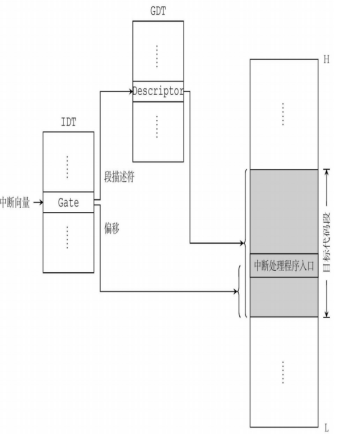
\includegraphics[width=12cm,height=11cm]{images/IDT.png}
        \caption{IDT寻址方式}
        \label{IDT寻址方式}
    \end{figure}
    
    $\bullet$ 建立IDT:IDT、IDTR的初始化与寻址方式与前面实验中的GDT、LDT类似,寻址方式见图\ref{IDT寻址方式}。
    
    \begin{lstlisting}[language={[x86masm]Assembler}]
; IDT
[SECTION .idt]
ALIGN	32
[BITS	32]
LABEL_IDT:
; 门                目标选择子,            偏移, DCount, 属性
%rep 255
		Gate	SelectorCode32, SpuriousHandler, 0, DA_386IGate
%endrep

IdtLen		equ	$ - LABEL_IDT
IdtPtr		dw	IdtLen - 1	; 段界限
		dd	0		; 基地址
; END of [SECTION .idt]
    \end{lstlisting}
    
    \begin{lstlisting}[language={[x86masm]Assembler}]
    ; 为加载 IDTR 作准备
    xor	eax, eax
    mov	ax, ds
    shl	eax, 4
    add	eax, LABEL_IDT		; eax <- idt 基地址
    mov	dword [IdtPtr + 2], eax	; [IdtPtr + 2] <- idt 基地址

    ; 加载 GDTR
	lgdt	[GdtPtr]

	; 关中断
	cli

	; 加载 IDTR
	lidt	[IdtPtr]
    \end{lstlisting}

    可以看到在IDT的初始化中,将255个描述符全部指向了同一个中断门SelectorCode32:SpuriousHandler,而这个中断处理程序的内容是在特定位置打印一个“!”:
    
    \begin{lstlisting}[language={[x86masm]Assembler}]
_SpuriousHandler:
    SpuriousHandler	equ	_SpuriousHandler - $$
	mov	ah, 0Ch				; 0000: 黑底    1100: 红字
	mov	al, '!'
	mov	[gs:((80 * 0 + 75) * 2)], ax	; 屏幕第 0 行, 第 75 列。
	xchg	bx, bx
	jmp	$
	iretd
    \end{lstlisting}


    $\bullet$ 初始化保护模式下的8259A:

\begin{lstlisting}[language={[x86masm]Assembler}]
; Init8259A -----------------------------------
Init8259A:
	mov	al, 011h
	out	020h, al	; 主8259, ICW1.
	call	io_delay

	out	0A0h, al	; 从8259, ICW1.
	call	io_delay

	mov	al, 020h	; IRQ0 对应中断向量 0x20
	out	021h, al	; 主8259, ICW2.
	call	io_delay

	mov	al, 028h	; IRQ8 对应中断向量 0x28
	out	0A1h, al	; 从8259, ICW2.
	call	io_delay

	mov	al, 004h	; IR2 对应从8259
	out	021h, al	; 主8259, ICW3.
	call	io_delay

	mov	al, 002h	; 对应主8259的 IR2
	out	0A1h, al	; 从8259, ICW3.
	call	io_delay

	mov	al, 001h
	out	021h, al	; 主8259, ICW4.
	call	io_delay

	out	0A1h, al	; 从8259, ICW4.
	call	io_delay

	mov	al, 11111110b	; 仅仅开启定时器中断
	;mov	al, 11111111b	; 屏蔽主8259所有中断
	out	021h, al	; 主8259, OCW1.
	call	io_delay

	mov	al, 11111111b	; 屏蔽从8259所有中断
	out	0A1h, al	; 从8259, OCW1.
	call	io_delay

	ret
; Init8259A ------------------------------------
\end{lstlisting}

    初始化的这些寄存器的结构在\ref{命令字设置}一节中已经详细说明,此处不再多做解释。可以看到在初始化ICW2时,将IRQ0$\sim$IRQ15对应到了20h$\sim$2Fh的位置,并且屏蔽了除了时钟中断以外所有的中断。不过由于我们将所有IDT描述符全都指向同一个打印程序,所以这些设定暂时没有体现出用处,他们将在\ref{调试时钟中断}中被用到。

    \subsubsection{调试程序\label{9a调试}}
    原始代码执行后结果如下图:
    \begin{figure}[H]
        \centering
        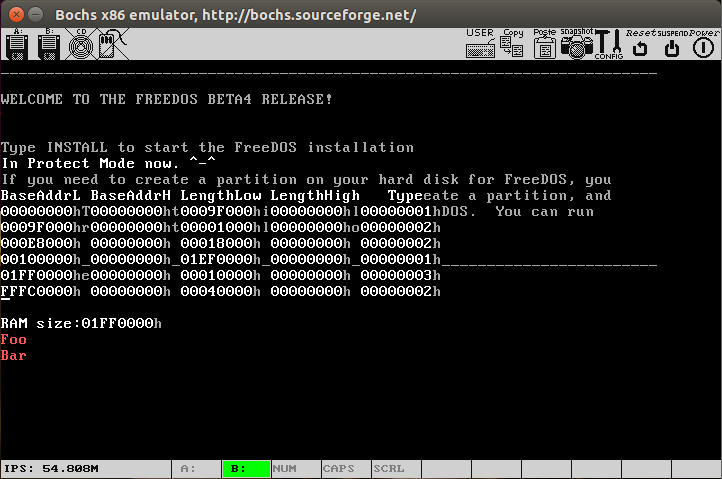
\includegraphics[width=12cm]{images/无!的输出.png}
        \caption{pmtest9a.asm执行结果}
        \label{无!的输出}
    \end{figure}
    %%% 解释
    
    在原始代码基础上进行以下修改:将关中断指令cli注释,并且在保护跳回实模式之前增加指令jmp \$使得程序停留在保护模式下,此时程序执行结果如下:
    \begin{figure}[H]
        \centering
        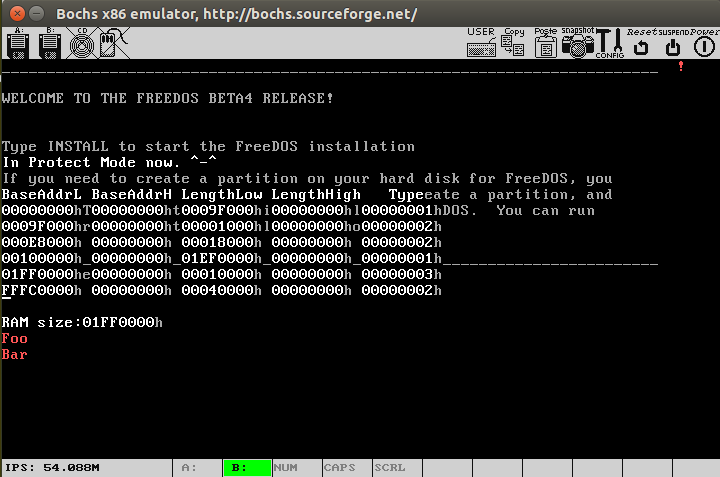
\includegraphics[width=12cm]{images/有!的输出.png}
        \caption{pmtest9a.asm修改后的执行结果}
        \label{有!的输出}
    \end{figure}
    
    %%% 解释

    在原始代码中,最后会返回到实模式,但是代码中并未在返回实模式后将8259A和应有的实模式中断处理还原回去,而仍然是保护模式下的设置,推测是由于在保护模式时中断处理程序并没有来得及执行,所以处于实模式的系统是无法正确识别保护模式下设置的中断处理程序并打印出的“!”的。第一次调试时,我们将断点设置在了SpuriousHandler中,但是并没有触发断点,推测是中断处理程序根本没有执行,从而发现了上述问题。故我们通过对pmtest9a作出如Listing~\ref{pmtest9a edited}的修改,即在保护模式下开中断并在最后增加jmp \$来使系统停在保护模式后,得到符合预期的结果,成功打印出了红色“!”。
    
    \begin{lstlisting}[language=diff, caption={使pmtest9a能正常显示叹号}, label={pmtest9a edited}]
--- a/i/pmtest9a.asm
+++ b/i/pmtest9a.asm
@@ -275,6 +275,9 @@ LABEL_SEG_CODE32:
 
        call    PagingDemo              ; 演示改变页目录的效果 
+       sti
+       jmp     $
+       ; 不返回实模式        
        ; 到此停止
        jmp     SelectorCode16:0

    \end{lstlisting}
    
    需要注意,pmtest9a.asm中并没有调用Init8259A,所以该程序中8259A的状态并不是我们设置的,是默认的全嵌套方式。我们不能确定最终打印出“!”一定是通过时钟中断产生的。
    
    \subsection{调试时钟中断例程\label{调试时钟中断}}
    \subsubsection{代码阅读}
    相较于pmtest9a,pmtest9的变化如下:
    
    $\bullet$ IDT初始化新增中断处理程序:
    
    \begin{lstlisting}[language={[x86masm]Assembler}]
; IDT
[SECTION .idt]
ALIGN	32
[BITS	32]
LABEL_IDT:
; 门                        目标选择子,            偏移, DCount, 属性
%rep 32
        Gate	SelectorCode32, SpuriousHandler,      0, DA_386IGate
%endrep
.020h:  Gate	SelectorCode32,    ClockHandler,      0, DA_386IGate
%rep 95
        Gate	SelectorCode32, SpuriousHandler,      0, DA_386IGate
%endrep
.080h:  Gate	SelectorCode32,  UserIntHandler,      0, DA_386IGate

IdtLen      equ	$ - LABEL_IDT
IdtPtr      dw	IdtLen - 1  ; 段界限
            dd	0           ; 基地址
; END of [SECTION .idt]
    \end{lstlisting}
    
    可以看到和pmtest9a相比,新增了20h号ClockHandler和80h号UserIntHandler,后者功能为向特定位置打印字符“I”,前者功能为在响应时钟中断的时候使后者打印的字符对应的ACSII值自增,来起到改变字符显示时钟变化的功能。
    
    \begin{lstlisting}[language={[x86masm]Assembler}]
_ClockHandler:
ClockHandler	equ	_ClockHandler - $$
	inc	byte [gs:((80 * 0 + 70) * 2)]	; 屏幕第 0 行, 第 70 列。
	mov	al, 20h
	out	20h, al				; 发送 EOI
	iretd

_UserIntHandler:
UserIntHandler	equ	_UserIntHandler - $$
	mov	ah, 0Ch				; 0000: 黑底    1100: 红字
	mov	al, 'I'
	mov	[gs:((80 * 0 + 70) * 2)], ax	; 屏幕第 0 行, 第 70 列。
	iretd
    \end{lstlisting}
    
    $\bullet$ IDTR和IMG的保存、实模式8259A的设置、使系统停在保护模式:
    
    \begin{lstlisting}[language={[x86masm]Assembler}]
    ; 保存 IDTR
	sidt	[_SavedIDTR]

	; 保存中断屏蔽寄存器(IMREG)值
	in	al, 21h
	mov	[_SavedIMREG], al
    \end{lstlisting}
    
    在加载GDTR和IDTR之前先将IDTR和IMG保存。
    
    \begin{lstlisting}[language={[x86masm]Assembler},caption={SetRealmode8259A}]
; SetRealmode8259A -----------------------------------
SetRealmode8259A:
	mov	ax, SelectorData
	mov	fs, ax

	mov	al, 017h
	out	020h, al	; 主8259, ICW1.
	call	io_delay

	mov	al, 008h	; IRQ0 对应中断向量 0x8
	out	021h, al	; 主8259, ICW2.
	call	io_delay

	mov	al, 001h
	out	021h, al	; 主8259, ICW4.
	call	io_delay

	mov	al, [fs:SavedIMREG]	; ┓恢复中断屏蔽寄存器(IMREG)的原值
	out	021h, al		;     ┛
	call	io_delay

	ret
; SetRealmode8259A ------------------------------------------------
    \end{lstlisting}
    
    设置好实模式下的中断处理机制。
    
    \begin{lstlisting}[language={[x86masm]Assembler}]
    call	Init8259A

	int	080h
	sti
	jmp	$
    \end{lstlisting}
    
    加入了sti(虽然在pmtest9中一开始就没有关中断,但是在关掉中断的pmtest9a中可以通过注释掉cli或者新增sti来解决\ref{9a调试}中的错误)和jmp \$使系统停在保护模式以便执行完80h号中断之后能看到20h号时钟中断的执行。
    
    \subsubsection{调试程序}
    %为了使结果更加明显可以通过同时自增地址的方式来打印,但是我太懒了暂时不想改
    直接运行原始代码,可以看到执行结果如下:
    \begin{figure}[H]
        \centering
        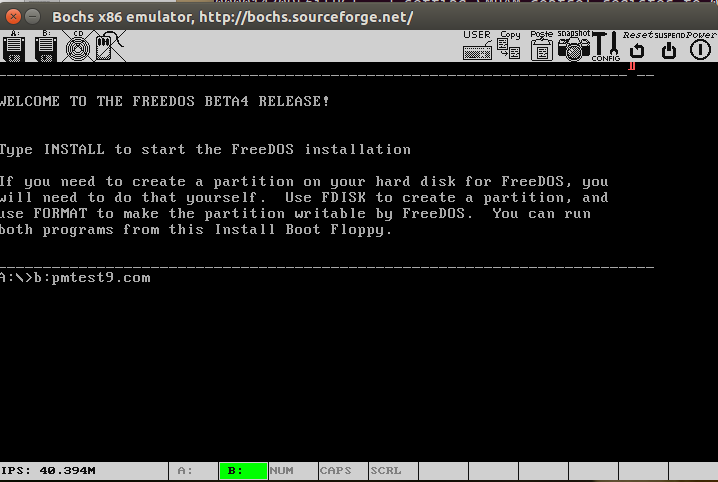
\includegraphics[width=12cm]{images/pmtest9执行结果.png}
        \caption{pmtest9执行结果}
        \label{pmtest9}
    \end{figure}
    
    不便于展示动图。事实上,第0行第75列处的字符是不停变化的,说明通过时钟中断int 20H,实现了值的自增,进而以字符的方式显示在屏幕上。同时,注意到我们看到的字符的变化并不是连续的,猜测是屏幕刷新频率低于时钟中断触发频率导致的。
    
    为了更好地理解程序,在ClockHandler和UserIntHandler中分别增加断点,重新编译、装载程序,并运行程序。停在第一个断点处时,执行结果如下:
    \begin{figure}[H]
        \centering
        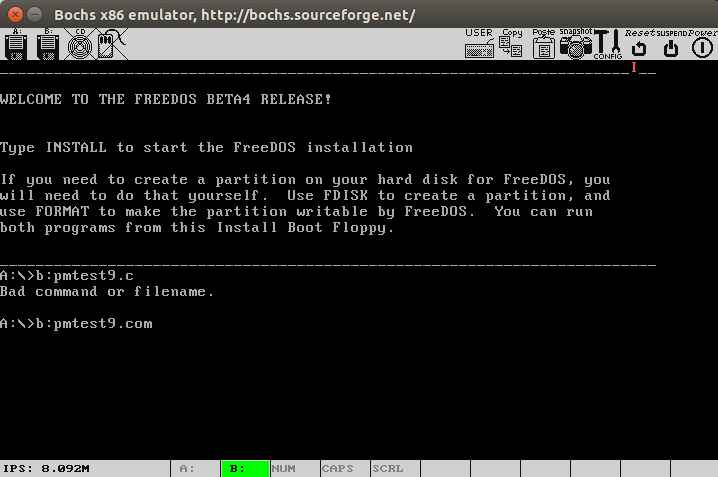
\includegraphics[width=12cm]{images/show_I.png}
        \caption{第一个断点——停在UserIntHandler}
        \label{breakpoint1}
    \end{figure}
    
    此时程序停在UserIntHandler,向低0行第70列写入一个I,屏幕上显示出对应的内容。继续执行程序,停在下一个断点。执行结果如下:
    \begin{figure}[H]
        \centering
        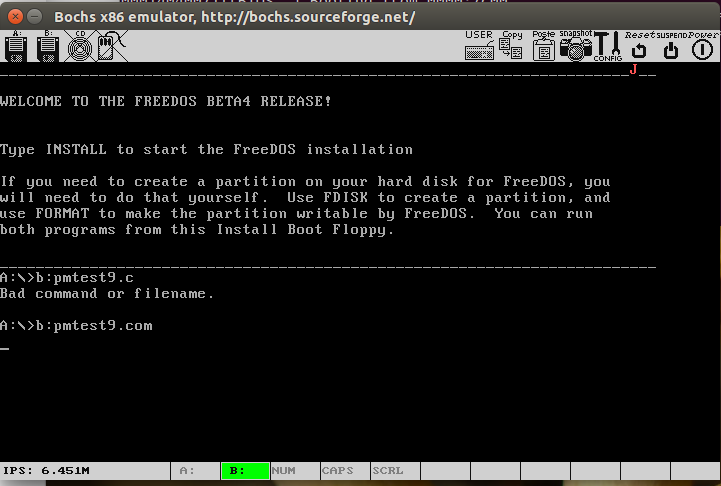
\includegraphics[width=12cm]{images/show_J.png}
        \caption{第二个断点——停在ClockHandler}
        \label{breakpoint2}
    \end{figure}
    
    事实上,程序一直在执行jmp \$,直到捕捉到下一个时钟中断,此时调用int 20H,完成自增。可以看到屏幕上指定位置的字符从I变成了J。继续调试,字符变成K,L,M等等。此处不再重复展示。
    
    调试结果与我们对代码的分析是一致的。
    
    
    \subsection{实现一个自定义的中断向量}
    
    我们一共实现了四个自定义中断向量,可以参见代码中的int.asm int2.asm int3.asm int4.asm这四个文件。其中前两个是保护模式下的中断,后两个是实模式下的中断。
    
    这四个中断的基本功能如下:
    
    $\bullet$ int.asm: 计时器中断。效果是屏幕上出现一个在 A 到 Z 间循环跳动的红色字符。一段时间后,循环结束,屏蔽中断,该字符会停止跳动,随后程序退出,返回DOS。
    
    $\bullet$ int2.asm:在int.asm的基础上,加上了键盘中断。因此除了不断跳动的字符以外,按下键盘时,屏幕上会出现通码;松开键盘时,屏幕上会出现断码。

    $\bullet$ int3.asm:修改实模式中断向量表,在实模式下实现了上面的键盘中断。
    
    $\bullet$ int4.asm:区别于int3.asm,同样修改了中断向量表,但在自定义功能完成后,将控制权交还给原本的处理程序,由原本的处理程序继续完成中断。效果是,程序退出后,在freedos下打字,除了像往常一样能正常输入外,还能在右上角看到一个会动的红色字符。
    
    \subsubsection{保护模式下自定义中断}
    
    我们将中断处理程序同一放置在handler.asm这个文件中,只要在主程序中引用这个文件,即可正确设置中断处理程序。
    
    首先,我们分析一下时钟中断的实现方式。原有时钟中断会不停的增加字符的值,造成字符值超过ASCII中字母的范围。所以我们为原有的时钟中断加入了循环功能,当 字符增加到Z时,将其重新设置为A。具体实现如Listing~\ref{handler1}所示,使用cmp byte比较字符,使用jz将字符重新设置为'A'或者增加字符的值。
    
    \begin{lstlisting}[language={[x86masm]Assembler}, caption={handler.asm}, label={handler1}]
_ClockHandler:
    push eax
    cmp byte [gs:CharPos], `Z`
    je .2
    inc byte [gs:CharPos]
    jmp .exit
.2:
    mov byte [gs:CharPos], `A`
.exit:
    mov al, 20h
    out 20h, al
    pop eax
    iretd
    ClockHandler equ _ClockHandler - $$
    \end{lstlisting}
    
    除此之外,我们还添加了一个自定义键盘中断处理程序。这个键盘中断处理程序会读取触发键盘中断的键值,并展示其扫描码。具体实现如Listing~\ref{handler2}所示,键盘中断位于中断描述符表的第21h号。键盘中断发生时,说明键盘的数据已经就绪。我们只需要读取键盘的数据端口(60h)即可得到键盘输入的数据。DispAL用于显示al中读取到的扫描码。ShowStr定义在utils.asm中,可以显示一个给定字符,str32定义为空格,故ShowStr str32用于显示空格。

    \begin{lstlisting}[language={[x86masm]Assembler}, caption={handler.asm}, label={handler2}]
_KeyBoardHandler:
    cli
    push eax
    
    in al, 60h
    call DispAL
    ShowStr str32

.exit:
    mov al, 20h
    out 20h, al
    pop eax
    iretd
KeyBoardHandler equ _KeyBoardHandler - $$
    \end{lstlisting}
    
    int2.asm的执行结果如图所示:
    
    \begin{figure}[H]
        \centering
        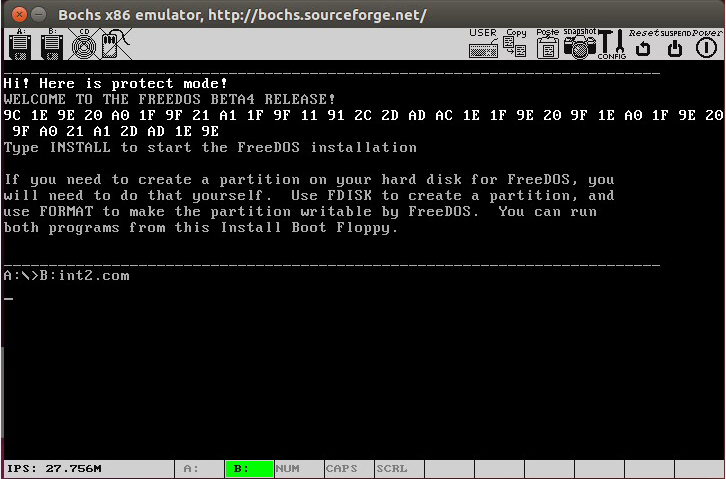
\includegraphics[width=12cm]{images/int2结果.png}
        \caption{int2程序执行结果}
        \label{int2}
    \end{figure}
    
    
    \subsubsection{实模式下自定义中断}

    实模式下的自定义中断可以直接通过写入中断向量表实现。实模式下的键盘中断位于中断向量表的第9号。故我们编写了新的9号中断,并把中断向量表指向这个新的中断。新的中断处理程序如Listing~\ref{int3}所示,由于需要在程序退出后,中断向量表仍然能够调用中断处理程序,所以我们需要将中断处理程序拷贝到内存中未被占用的位置,这里选择了 0x200 这个位置。中断处理程序的实现与保护模式下大致相同,可以循环显示从A-Z的红色字符。
    
    \begin{lstlisting}[language={[x86masm]Assembler}, caption={int3.asm}, label={int3}]
    _int9:
    push eax
    push gs
    mov ax, 0b800h
    mov gs, ax
    in al, 60h ; 读取缓冲区
    cmp byte [gs:((80 * 0 + 70) * 2)], `Z`
    je .2
    inc byte [gs:((80 * 0 + 70) * 2)]
    jmp .exit
.2:
    mov byte [gs:((80 * 0 + 70) * 2)], `A`
.exit:
    mov al, 20h
    out 20h, al ; 输出 EOI
    pop gs
    pop eax
    iret
    \end{lstlisting}
    
    在此基础上,我们在int4.asm中添加了保存原有9号中断,以及重定向到原有9号中断的功能,使得在发生键盘中断以后,除了能够实现输入功能,还能够在右上角显示一个变化的红色字符。
    
    \begin{lstlisting}
_int9:
    push ax
    push gs
    ; 运行自定义的中断程序
    mov ax, 0b800h
    mov gs, ax
    mov byte [gs:(CharPos + 1)], 0Ch
    inc byte [gs:CharPos]
    jmp .exit
.exit:
    pop gs
    pop ax
    ; 由原本的中断程序接管
    ; jmp dword 60h:0d0d6h
    push word [cs:202h]
    push word [cs:200h]
    retf
    \end{lstlisting}
    
    int4.asm的执行结果如图~\ref{示例1}和图~\ref{示例2}所示:
    \begin{figure}[H]
        \centering
        \begin{minipage}[t]{0.5\textwidth}
        \centering
        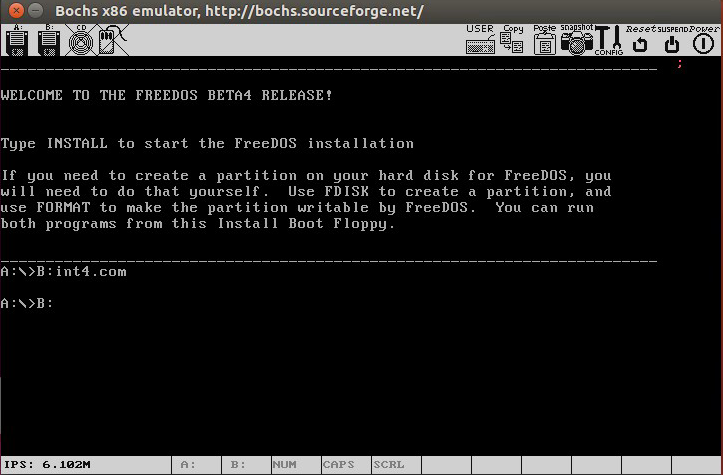
\includegraphics[width=7cm]{images/int4结果1.png}
        \caption{int4运行结果1}
        \label{示例1}
        \end{minipage}
        \begin{minipage}[t]{0.49\textwidth}
        \centering
        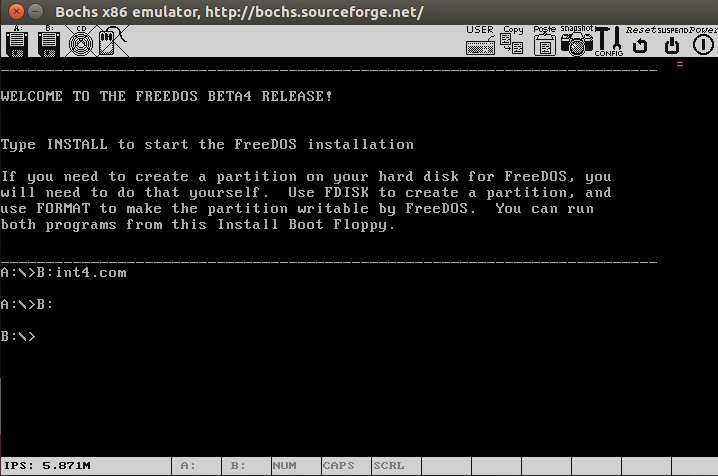
\includegraphics[width=7cm]{images/int4结果2.png}
        \caption{int4运行结果2}
        \label{示例2}
        \end{minipage}
    \end{figure}
    
    
    \section{实验结果总结}
    \subsection{中断和异常的概念}
    早期中断和异常都被称为中断,后来按照产生的原因进行了区分。异常和中断都是软件或者硬件发生了某种情形而通知处理器的行为。
    \subsubsection{异常}
    异常也叫内部中断,它不需要硬件支持。异常的引入表示CPU执行指令时本身出现的问题。异常可分为以下三种类型:
    
    $\bullet$ Fault:一种可以被更正的异常。而且一旦被更正,程序可以不失连续性地继续执行。当一个fault发生,处理器会把产生fault指令之前的状态保存起来,异常处理程序的返回地址将会是产生fault的指令,而不是其后的那条指令。
    
    $\bullet$ Trap:是一种在发生trap的指令执行之后立即被报告的异常,它也允许程序或任务不失连续性地继续执行。异常处理程序的返回地址将会是产生trap的指令之后的那条指令。
    
    $\bullet$ Abort:是一种不总是报告准确异常发生位置的异常,它不允许程序或者任务继续执行,而是用来报告严重错误的。
    
    注意,异常是同步的,这是指异常发生的时候,CPU立即处理本次异常,直到异常处理结束之后才能继续进行接下来的任务。
    
    \subsubsection{中断}
    这里的中断指的是外部中断。中断的引入是为了支持CPU和设备之间的并行操作。中断可以分为可屏蔽中断和不可屏蔽中断。
    
    $\bullet$ 可屏蔽中断:指通过可屏蔽中断请求线INTR向CPU发出中断请求,CPU可以通过在中断控制器中设置响应的屏蔽字来屏蔽他或不屏蔽他,被屏蔽的中断请求将不被送至CPU。
    
    $\bullet$ 不可屏蔽中断:指通过专门的不可屏蔽请求线NMI向CPU发出的中断请求,通常是非常紧急的硬件故障。
    
    注意,外部中断是异步的,意思是所有中断来的信号都是记录在中断寄存器中的,当CPU执行完一道指令之后,如果是开中断状态,则会检查中断寄存器中有没有中断,如果有中断,就会选择一个中断优先级比较高的中断先处理,等到处理完中断再继续执行;如果是关中断,则不会检查,而直接执行下一条指令。
    
    \subsection{处理机制}
    \subsubsection{实模式下的中断处理}
    实模式下,中断转移方法与8086相同,即通过中断向量号直接去中断向量表种找到中断处理程序入口,然后跳转到指定位置执行中断处理程序。示意图如下:
    \begin{figure}[H]
        \centering
        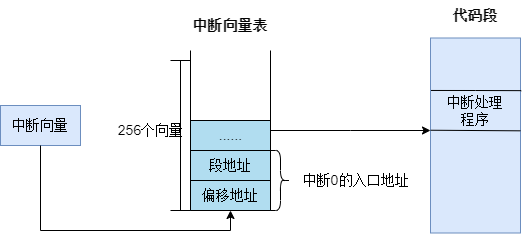
\includegraphics[width=12cm]{images/实模式处理.png}
        \caption{实模式中断处理}
        \label{实模式中断处理}
    \end{figure}
    
    \subsubsection{保护模式下的中断处理}
    不同于实模式,在保护模式下,中断向量表被IDT代替。IDT的作用是将每一个中断向量和一个描述符对应起来。IDT的描述符有以下三类:中断门描述符、陷阱门描述符、任务门描述符。
    
    $\bullet$ 中断门和陷阱门
    中断门和陷阱门的结构如下图所示:
    \begin{figure}[H]
        \centering
        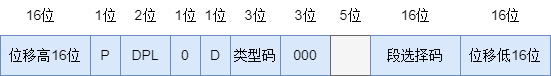
\includegraphics[width=14cm]{images/中断门结构.png}
        \caption{中断门、陷阱门结构}
        \label{中断门结构}
    \end{figure}
    
    其中灰色部分表示保留,不使用。其中段选择码和偏移用来定位中断处理程序,其余标志该描述符的属性。具体的处理机制如图\ref{中断门和陷阱门}。
    
    \begin{figure}[H]
        \centering
        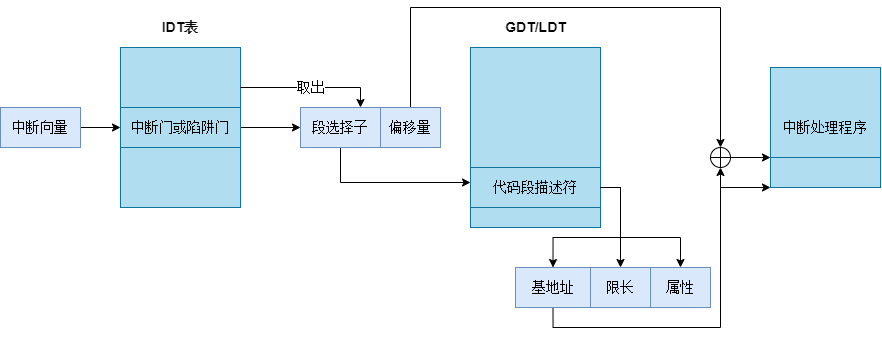
\includegraphics[width=14cm]{images/陷阱门处理机制.png}
        \caption{中断门和陷阱门}
        \label{中断门和陷阱门}
    \end{figure}
    
    注意,中断门和陷阱门的区别是对中断允许标志IF位的影响。中断门向量引起中断时会复位IF,此时其他中断干扰会被屏蔽,最终通过iret从堆栈上恢复出IF的原值。
    
    $\bullet$ 任务门
    
    任务门的结构如下图所示:
    \begin{figure}[H]
        \centering
        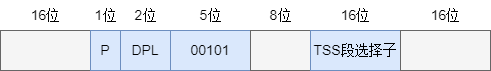
\includegraphics[width=12cm]{images/任务门结构.png}
        \caption{任务门结构}
        \label{任务门结构}
    \end{figure}
    
    同样,灰色部分表示空闲不使用。任务门不需要提供段内偏移,因为任务门不指向某一个子程序的入口,TSS本身是作为一个段来对待的。任务门的处理机制如下图。
    
    \begin{figure}[H]
        \centering
        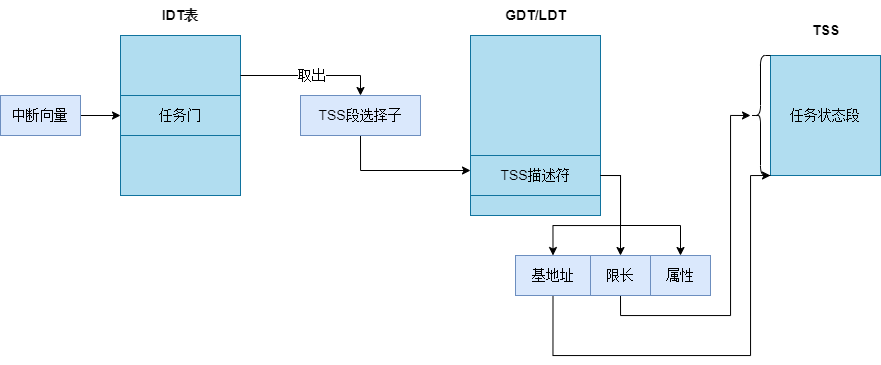
\includegraphics[width=15cm]{images/任务门.png}
        \caption{任务门}
        \label{任务门}
    \end{figure}
    
    根据TSS段的信息转入对应的中断或异常处理程序。
    
    \subsection{8259A的工作原理}
    \subsubsection{8259A的内部结构}
    8259A的内部结构如图\ref{8259A内部结构}所示。
    \begin{figure}[H]
        \centering
        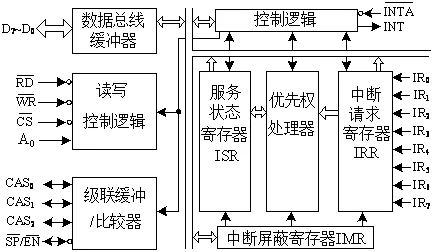
\includegraphics[width=10cm]{images/8259A内部结构.png}
        \caption{8259A内部结构}
        \label{8259A内部结构}
    \end{figure}
    
    关于各个组成部分的解释如下:
    
    $\bullet$ 中断请求寄存器IRR(Interrupt Request Register)

    外部8级中断请求信号从IR7~IR0脚上引入,有请求时相应位置为1。多个中断请求可同时进入。中断请求信号可为高电平或上升沿触发,通过编程定义。
    
    $\bullet$ 中断屏蔽寄存器IMR(Interrupt Mask Register)
    
    存放中断屏蔽信息,每1位与1个IR位对应,置1表示禁止对应中断请求进入系统。用来有选择地禁止某些设备请求中断。
    
    $\bullet$ 服务状态寄存器ISR(Interrupt Service Register)
    
    保存正处理的中断请求。任一中断被响应而执行其服务程序时,相应位置1,直到处理结束。若有多重中断的情况,会有多个位置为1。
    
    $\bullet$ 优先级处理器PR(Priority Resolver)
    
    判别请求寄存器IRR里中断的优先级,把优先级最高的中断请求选进服务寄存器ISR中。多重中断出现时,PR判定新出现的中断能否去打断正在处理的中断,优先服务更高的中断级别。
    
    $\bullet$ 控制电路
    
    它包含一组初始化命令字寄存器$ICW_1 \sim  ICW4$ 和一组操作命令字寄存器$OCW_1 \sim OCW_3$,管理8259A的全部工作。控制电路根据IRR设置和PR判定,决定控制信号,然后从INT脚向CPU发中断请求信号,接收CPU或总线控制器8288送来的中断响应信号$\overline{INTA}$。中断响应时ISR相应位置1,并发送中断类型号n,经数据总线缓冲器送到D7$\sim$D0;中断服务程序结束时,按编程规定方式结束中断。
    
    $\bullet$ 数据总线缓冲器
    
    是8259A与CPU的接口,CPU经它向8259A写控制字,接收8259A送出的中断类型号,还可从中读出状态字(中断请求、屏蔽、服务寄存器的状态)和中断查询字。
    
    $\bullet$ 读写控制逻辑
    
    接收CPU的$\overline{RD}$、$\overline{WR}$、地址、片选。一片8259A只占两个I/O地址,XT机中A0接地址A0,口地址为20H、21H。当与8086 连时,A0脚接地址A1,A0的0/1选偶/奇地址口。执行OUT指令时,$\overline{WR}$信号与A0配合,将控制字写入ICW和OCW寄存器;
    执行IN指令时,$\overline{RD}$信号与A0配合,将内部寄存器的内容经D7~D0送给CPU。
    
    $\bullet$ 级联缓冲/比较器
    
    一片8259A最多引入8级中断,超过8级要用多片8259A构成主从关系,级联使用。当需要用两片8259A:从片输出INT接主片$IR_i$,主从片的3条级联信号线CAS2$\sim$CAS0并接。
    
    \subsubsection{8259A的工作方式}
    写入初始化命令字ICW和控制命令字OCW,可以对8259A设置不同的工作方式。
    
    $\bullet$ 设置优先级方式
    
    优先级方式分为以下几种:
    
    $\cdot$ 全嵌套方式:最基本方式,初始化后自动进入。
    
    从各IRi脚引入的中断请求具有固定优先级,$IR_0 \rightarrow IR7$依次降低,$IR_0$ 最高。8259A初始化后自动进入此方式。处理过程中,高级中断打断低级中断,禁止低级或同级中断进入。
    
    $\cdot$ 特殊全嵌方式
    
    同全嵌套方式,但允许同级中断进入(在主片看来,从片的8级中断为同级中断)。
    
    $\cdot$ 优先级自动循环方式
    
    各中断请求优先级相同,$IR_i$服务完后成为最低级,$IR_{i+1}$成最高级。初始优先级从高到低为$IR_0 \rightarrow IR_7$。
    
    $\cdot$ 优先级特殊循环方式
    
    也称为设置最低优先级方式,与优先级自动循环方式类似,只是最低优先级由程序设置,并非$IR_7$最低。$IR_i$设为最低后,$IR_i+1$便是最高。
    
    $\bullet$ 中断屏蔽方式
    
    开中断情况下,可将中断屏蔽寄存器IMR的相应位置1,来屏蔽某一级或某几级中断。代码实现上,可用CLI指令关中断,禁止可屏蔽中断进入。有两种屏蔽方式:普通屏蔽方式和特殊屏蔽方式。
    
    $\bullet$ 结束中断方式
    
    中断响应后,ISR的相应位$IS_n$置1,中断结束后应将$IS_n$清0,表示结束中断。有2种结束中断方式:自动和非自动,后者又分普通结束和特殊结束(EOI和SEOI)。这里不再展开详述。
    
    $\bullet$ 中断查询方式
    
    使用一条IN指令读取中断查询字,就可查到8259A是否有中断请求以及哪个优先级最高。
    
    \subsubsection{8259A的命令字设置\label{命令字设置}}
    为使8259A按预定方式工作,必须对它编程,由CPU向其控制寄存器发各种控制命令。控制命令分为两类——初始化命令字和操作命令字。
    
    $\bullet$ 初始化命令字
    
    初始化命令字的写入流程如下图所示。
    \begin{figure}[H]
        \centering
        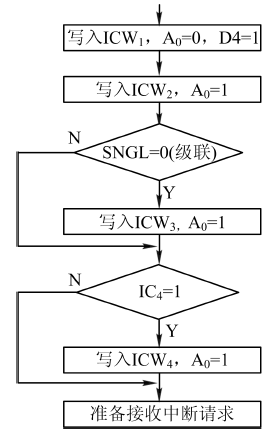
\includegraphics[width=5cm]{images/初始化命令字.png}
        \caption{初始化命令字写入流程}
        \label{初始化命令字写入流程}
    \end{figure}
    
    初始化命令字必须从$ICW_1$开始顺序写入规定端口,级联时要写入$ICW_3$,无级联时无需写入。
    
    $\cdot$ $ICW_1$——初始化字
    
    $ICW_1$的结构如下图:
    \begin{figure}[H]
        \centering
        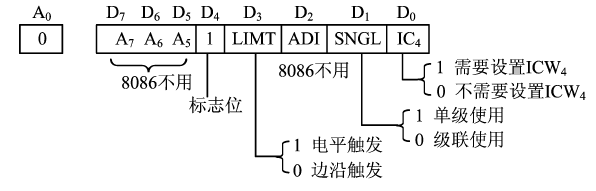
\includegraphics[width=12cm]{images/ICW1.png}
        \caption{ICW1结构}
        \label{ICW1}
    \end{figure}
    
    $A_0$=0,$ICW_1$写入偶地址口;$D_1$表示SNGL属性,标志是否使用级联。级联时SNGL=0, 要写入$ICW_3$。
    
    $\cdot$ $ICW_2$——中断向量码
    
    $ICW_2$的结构如下图:
    \begin{figure}[H]
        \centering
        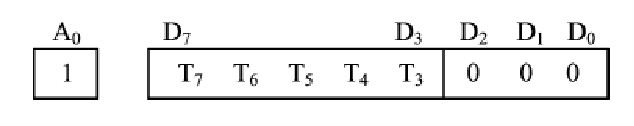
\includegraphics[width=12cm]{images/ICW2.png}
        \caption{ICW2结构}
        \label{ICW2}
    \end{figure}
    
    $A_0$=1,$ICW_2$写入奇地址口;T7$\sim$T3位用于确定中断类型码n的高5位,低3位D2$\sim$D0则由8259A根据从IRi上引入中断的引脚序号自动填入,从IR0$\sim$IR7的序号依次为000~111,其初值可以置为0。$ICW_2$的高5位内容是可以任选的,一旦高5位确定,一块芯片的8个中断请求信号IR0$\sim$IR7的中断类型号也就确定了。
    
    $\cdot$ $ICW_3$——级联控制字
    
    $ICW_3$只在级联时使用。$ICW_3$的格式和8259A主从结构连接示意图如下:
    \begin{figure}[H]
        \centering
        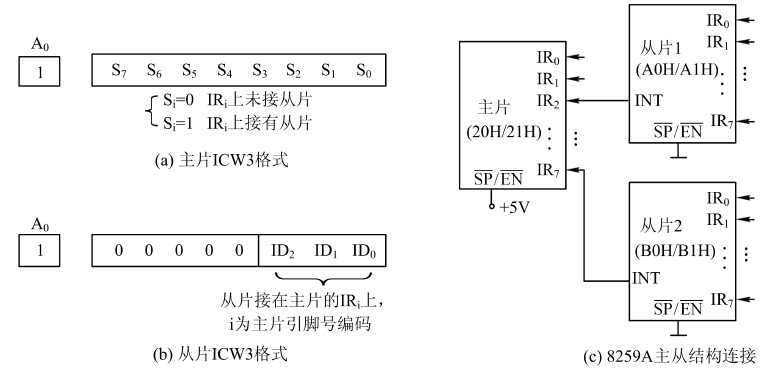
\includegraphics[width=14cm]{images/ICW3.png}
        \caption{ICW3结构以及主从结构}
        \label{ICW3}
    \end{figure}
    
    主片$ICW_3$格式:$S_i$=0,$IR_i$上未接从片,$S_i$=1接有从片。
    从片$ICW_3$格式。低3位指明从片接主片哪个引脚,$ID_2 \sim ID0$ = 000 $\sim$ 111表示$IR_0$ $\sim$ $IR_7$引脚。
    
    $\cdot$ $ICW_4$——中断结束方式字
    
    8086系统$ICW_4$必须设置,写入奇地址口。$ICW_4$的结构如下:
    \begin{figure}[H]
        \centering
        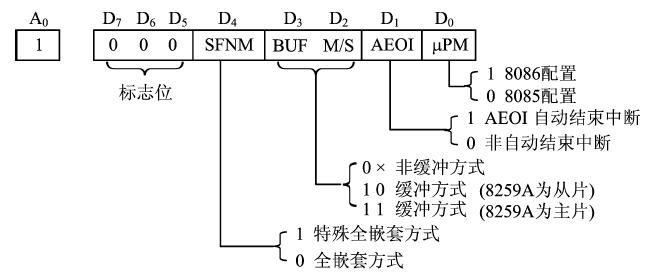
\includegraphics[width=12cm]{images/ICW4.png}
        \caption{ICW4结构}
        \label{ICW4}
    \end{figure}
    
    $\bullet$ 操作命令字
    
    用来改变8259A的中断控制方式,屏蔽中断源,以及读出8259A的工作状态(IRR,ISR,IMR),初始化完成后任意状态皆可写入,顺序也没有严格要求,但是对端口地址有规定:$OCW_1$奇地址端口(A0=1),$OCW_2$,$OCW_3$必须为偶地址端口。
    
    $\cdot$ $OCW_1$——中断屏蔽字
    
    直接对中断屏蔽寄存器IMR的各位进行置1或清0。当$M_i$位置1,相应IRi的中断请求将被屏蔽,清0则允许中断。其结构如下:
    
    \begin{figure}[H]
        \centering
        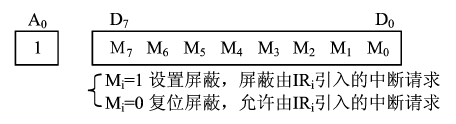
\includegraphics[width=12cm]{images/OCW1.png}
        \caption{OCW1结构}
        \label{OCW1}
    \end{figure}
    
    $\cdot$ $OCW_2$——优先级循环和中断结束
    
    $OCW_2$ 是设置优先级循环方式和中断结束方式的命令字。其结构如下:
    \begin{figure}[H]
        \centering
        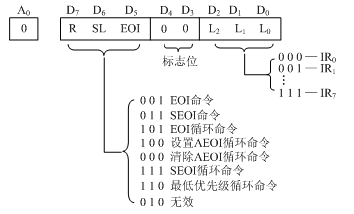
\includegraphics[width=12cm]{images/OCW2.png}
        \caption{OCW2结构}
        \label{OCW2}
    \end{figure}
    
    $\cdot$ $OCW_3$——屏蔽方式和状态读出控制字
    
    $OCW_3$的结构如下图:
    \begin{figure}[H]
        \centering
        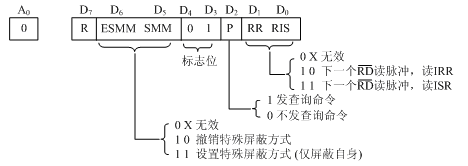
\includegraphics[width=12cm]{images/OCW3.png}
        \caption{OCW3结构}
        \label{OCW3}
    \end{figure}
    
    \subsubsection{8259A工作原理概述}
    
    先通过$ICW_1$ $\sim$ $ICW_4$来初始化8259A,使芯片处于一个规定的基本工作方式。初始化完成后,开中断,一个外部中断请求信号通过中断请求线IRQ,传输到IMR(中断屏蔽寄存器),IMR根据所设定的中断屏蔽字($OCW_1$),决定是将其丢弃还是接受。
    
    如果可以接受,则8259A将IRR(中断请求暂存寄存器)中代表此IRQ的位置位,以表示此IRQ有中断请求信号,并同时向CPU的$\overline{INTR}$管脚发送一个信号,但CPU这时可能正在执行一条指令,因此CPU不会立即响应,而当这CPU正忙着执行某条指令时,还有可能有其余的IRQ线送来中断请求,这些请求都会接受IMR的挑选,如果没有被屏蔽,那么这些请求也会被放到IRR中,也即IRR中代表它们的IRQ的相应位会被置1。
    
    当CPU执行完一条指令时后,会检查一下$\overline{INTR}$管脚是否有信号,如果发现有信号,就会转到中断服务,此时,CPU会立即向8259A芯片的INTA(中断应答)管脚发送一个信号。当芯片收到此信号后,判优部件开始工作,它在IRR中,挑选优先级最高的中断,将中断请求送到ISR(中断服务寄存器),也即将ISR中代表此IRQ的位置位,并将IRR中相应位置零,表明此中断正在接受CPU的处理。同时,将它的编号写入中断向量寄存器IVR的低三位。这时,CPU还会送来第二个INTA信号,当收到此信号后,芯片将IVR中的内容,也就是此中断的中断号送上通向CPU的数据线。
    
    \subsection{中断号的处理向量初始化}
    本节从linux源码角度阐述中断号的处理向量初始化。
    
    在linux系统中,中断一共有256个,0~19主要用于异常与陷阱,20~31是intel保留,未使用。32~255作为外部中断进行使用。特别的,0x80中断用于系统调用。机器上电时,BIOS会初始化一个中断向量表,当交接给linux内核后,内核会自己新建立一个中断向量表,之后完全使用自己的中断向量表,舍弃BIOS的中断向量表。
    
    中断的初始化大体上分为两个部分,第一个部分为汇编代码的中断向量表的初次初始化,第二部分为C语言代码,又分为异常与陷阱的初始化和中断的初始化。
    \begin{figure}[H]
        \centering
        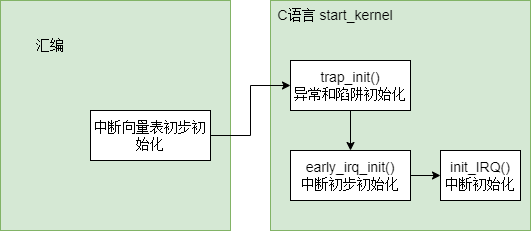
\includegraphics[width=12cm]{images/中断初始化.png}
        \caption{中断初始化}
        \label{中断初始化}
    \end{figure}
    
    在汇编的中断向量表初始化过中,主要对整个中断向量表进行了初始化,其主要工作是:
    $\cdot$ 所有的门描述符的权限位为0;
    $\cdot$ 所有的门描述符的段选择符为\_\_KERNEL\_CS;
    $\cdot$ 0$\sim$31的门描述符的中断处理程序为early\_idt\_handlers[i](0 <= i <= 31);
    $\cdot$ 其他的门描述符的中断处理程序为ignore\_int。
    
    trap\_init()所做的异常与陷阱初始化,就是修改中断向量表的前19项(异常和中断),主要修改他们的中断处理函数入口和权限位,特殊的如任务门还会设置它们的段选择符。在trap\_init()中就已经把所有的异常和陷阱都初始化完成了,并会把新的中断向量表地址放入IDTR寄存器,开始使用新的中断向量表。
    
    在early\_irq\_init()中,主要工作是初始化整个中断描述符表,将数组中的每个中断描述符中的必要变量进行初始化。
    
    最后在init\_IRQ()中,主要工作是初始化中断向量表中的所有中断门描述符,对于一般的中断,内核将它们的中断处理函数入口设置为interrupt[i],而一些特殊的中断会在apic\_intr\_init()中进行设置。之后,init\_IRQ()会初始化内部和外部的中断控制器,最后将一般的中断使用的中断控制器设置为8259A,中断处理函数为handle\_level\_irq(电平触发)。
    
    \subsection{建立IDT}
    
    参考\ref{调试时钟中断}节中关于IDT的内容,IDT是按地址顺序从0h号开始顺序设置描述符的,也就是说假设你要设置20h号中断,你只需要设置好第20个描述符,将其指向32位代码段中的中断处理程序。
    
    \subsection{控制时钟中断}
    可以通过修改8259A的状态来控制时钟中断。
    \begin{figure}[H]
        \centering
        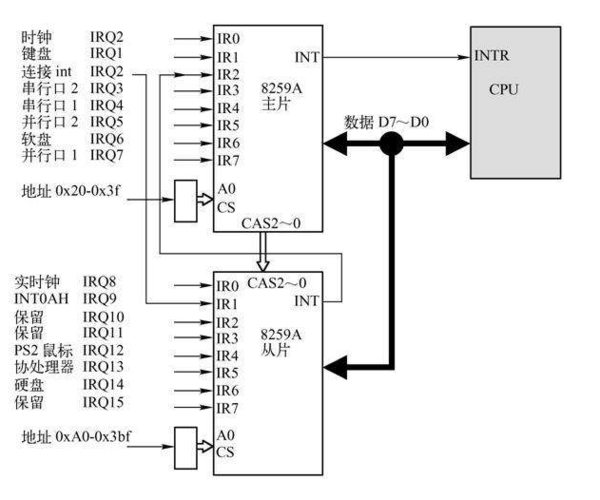
\includegraphics[width=10cm]{images/2_8259A.png}
        \caption{主从8259A}
        \label{主从8259A}
    \end{figure}
    从主从8259A结构中可以看到,时钟中断处在8259A主片的IR0端口。通过$OCW_1$可以设置主片的$IR_0$是否屏蔽,从而决定系统对时钟中断是否响应。
    
    时钟中断的中断处理程序位于IDT的第20h号,修改IDT中对应位置即可将时钟中断的处理定位到自定义程序。
    
    Q:为什么时钟中断时候,没有看到int的指令?
    
    int指令触发的是软中断。而时钟中断是由定时器触发的中断,即硬件中断。时钟中断是由8259A直接发送给CPU进行处理的,不需要int指令来触发。
    
    \subsection{IOPL的作用与基本机理}
    \subsubsection{IOPL的作用}
    IOPL是I/O保护机制的关键之一,它能够控制I/O的权限。IOPL保存在寄存器eflags的12、13位。
    \begin{figure}[H]
        \centering
        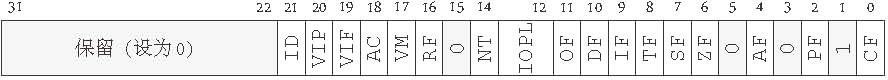
\includegraphics[width=14cm]{images/IOPL.png}
        \caption{eflags结构}
        \label{eflags}
    \end{figure}
    
    指令in,ins,out,outs,cli,sti必须在CPL$\leq$IOPL的条件下才能执行。上述指令是I/O敏感指令,如果低特权级的指令试图访问这些指令会导致常规保护错误。
    
    \subsubsection{IOPL的基本机理}
    处理器不限制0特权级程序的I/O访问,它总是允许的。但是,可以限制低特权级程序的I/O访问权限。这是很重要的,操作系统的功能之一是设备管理,它可能不希望应用程序拥有私自访问外设的能力。
    
    可以改变IOPL的指令只有popf和iretd,但只有运行在ring0的程序才能将其改变。运行在低特权级下的程序无法改变IOPL,不 过,如果试图那样做的话并不会产生任何异常,只是IOPL不会改变,仍然保持原样。
    
    另一个与I/O操作特权级有关的概念是I/O位图。I/O位图基址是一个以TSS的地址为基址的偏移,指向的便是I/O许可位图。之所以叫做位图,是因为它的每一位表示一个字节的端口地址是否可用。如果某一位为0,则表示此位对应的端口号可用,为1则不可用。由于每一个任务都可以有单独的TSS,所以每一个任务可以有它单独的I/O许可位图。
    
    IO位图与IOPL是或的关系,即只要满足一个条件即可。
    
    \begin{table}[H]
    \centering
    \begin{tabular}{|c|c|c|}
    \hline
    {\color[HTML]{333333} \textbf{指令}} & \textbf{功能} & \textbf{条件}                  \\ \hline
    cli                                & 清除IF位       & CPL\textless{}=IOPL          \\ \hline
    sti                                & 设置IF位       & CPL\textless{}=IOPL          \\ \hline
    in                                 & 从IO读数据      & CPL\textless{}=IOPL 或 IO位图许可 \\ \hline
    ins                                & 从IO读字符串     & CPL\textless{}=IOPL 或 IO位图许可 \\ \hline
    out                                & 向IO写数据      & CPL\textless{}=IOPL 或 IO位图许可 \\ \hline
    outs                               & 向IO写字符串     & CPL\textless{}=IOPL 或 IO位图许可 \\ \hline
    \end{tabular}
    \end{table}
    
    \section{各人实验贡献与体会}
    本次实验主要探究了异常与中断的实现。在汇编语言课程中,我们就已经对实模式下的中断有了一定的认识,本次重点关注了保护模式下的异常中断处理机制。通过对pmtest9a.asm的调试,熟悉了IDT的建立以及保护模式下中断调用;通过对pmtest9.asm的调试,理解了时钟中断的触发机理。最后,基于对中断原理的理解,我们编写了实模式和保护模式下自定义中断(键盘中断和计时器中断)。在实验过程中,组员之间积极讨论,对原理有了更深刻的理解。
    
    实验分工如下:李心杨负责撰写自定义中断程序的说明,协助其他同学解决代码中的问题;王宇骥对中断原理进行总结,完善报告细节;林锟扬负责编写自定义中断程序;郑炳捷负责调试pmtest9a.asm并完成对应部分实验报告。
    
    
    
    \section*{参考资料汇总}
    \begin{enumerate}
        \item 配套教材《Orange's 一个操作系统的实现》。
        \item 微机系统课程PPT 《8.2 8259A的原理》。
        \item \href{
        https://www.cnblogs.com/mainull/p/7821255.html}{任务门、中断门、陷阱门和调用门 - silenccfly -博客园}。
        \item \href{https://blog.csdn.net/HizT_1999/article/details/106989155}{操作系统——认识认识保护模式(三)中断}。
        \item \href{https://www.cnblogs.com/alwaysking/p/12348016.html}{汇编学习笔记(21) - IO 保护}。
    \end{enumerate}
    
    
    \begin{table}[H]
    \centering
    \begin{tabular}{|p{4cm}<{\centering}|p{6cm}<{\centering}|p{3cm}<{\centering}|}
    \hline
    \multicolumn{3}{|c|}{\textbf{教师评语}}                                                  \\ \hline
    \multicolumn{3}{|c|}{ \rule{0pt}{60pt} }                                                      \\ \hline
    {\textbf{姓名}} & {\textbf{学号}}   & \textbf{分数} \\ \hline
    \multicolumn{1}{|c|}{李心杨} & \multicolumn{1}{c|}{2020302181022}  &             \\ \hline
    \multicolumn{1}{|c|}{王宇骥} & \multicolumn{1}{c|}{2020302181008} &             \\ \hline
    \multicolumn{1}{|c|}{林锟扬} & \multicolumn{1}{c|}{2020302181032} &             \\ \hline
    \multicolumn{1}{|c|}{郑炳捷} & \multicolumn{1}{c|}{2020302181024} &             \\ \hline
    \multicolumn{3}{|l|}{教师签名:}       \\ 
    \multicolumn{3}{|r|}{} \\ 
    \multicolumn{3}{|r|}{年 \space 月 \space 日} \\ \hline
    \end{tabular}
    \end{table}
    
\end{document}